% 若编译失败,且生成 .synctex(busy) 辅助文件,可能有两个原因:
% 1. 需要插入的图片不存在:Ctrl + F 搜索 'figure' 将这些代码注释/删除掉即可
% 2. 路径/文件名含中文或空格:更改路径/文件名即可

% ------------------------------------------------------------- %
% >> ------------------ 文章宏包及相关设置 ------------------ << %
% 设定文章类型与编码格式
\documentclass[UTF8]{report}		

% 本文特殊宏包
\usepackage{siunitx} % 埃米单位

% 本 .tex 专属的宏定义
    \def\V{\ \mathrm{V}}
    \def\mV{\ \mathrm{mV}}
    \def\kV{\ \mathrm{KV}}
    \def\KV{\ \mathrm{KV}}
    \def\MV{\ \mathrm{MV}}
    \def\A{\ \mathrm{A}}
    \def\mA{\ \mathrm{mA}}
    \def\kA{\ \mathrm{KA}}
    \def\KA{\ \mathrm{KA}}
    \def\MA{\ \mathrm{MA}}
    \def\O{\ \Omega}
    \def\mO{\ \Omega}
    \def\kO{\ \mathrm{K}\Omega}
    \def\KO{\ \mathrm{K}\Omega}
    \def\MO{\ \mathrm{M}\Omega}
    \def\Hz{\ \mathrm{Hz}}

% 自定义宏定义
    \def\N{\mathbb{N}}
    \def\F{\mathbb{F}}
    \def\Z{\mathbb{Z}}
    \def\Q{\mathbb{Q}}
    \def\R{\mathbb{R}}
    \def\C{\mathbb{C}}
    \def\T{\mathbb{T}}
    \def\S{\mathbb{S}}
    \def\A{\mathbb{A}}
    \def\I{\mathscr{I}}
    \def\Im{\mathrm{Im\,}}
    \def\Re{\mathrm{Re\,}}
    \def\d{\mathrm{d}}
    \def\p{\partial}

% 导入基本宏包
    \usepackage[UTF8]{ctex}     % 设置文档为中文语言
    \usepackage[colorlinks, linkcolor=blue, anchorcolor=blue, citecolor=blue, urlcolor=blue]{hyperref}  % 宏包:自动生成超链接 (此宏包与标题中的数学环境冲突)
    % \usepackage{hyperref}  % 宏包:自动生成超链接 (此宏包与标题中的数学环境冲突)
    % \hypersetup{
    %     colorlinks=true,    % false:边框链接 ; true:彩色链接
    %     citecolor={blue},    % 文献引用颜色
    %     linkcolor={blue},   % 目录 (我们在目录处单独设置),公式,图表,脚注等内部链接颜色
    %     urlcolor={orange},    % 网页 URL 链接颜色,包括 \href 中的 text
    %     % cyan 浅蓝色 
    %     % magenta 洋红色
    %     % yellow 黄色
    %     % black 黑色
    %     % white 白色
    %     % red 红色
    %     % green 绿色
    %     % blue 蓝色
    %     % gray 灰色
    %     % darkgray 深灰色
    %     % lightgray 浅灰色
    %     % brown 棕色
    %     % lime 石灰色
    %     % olive 橄榄色
    %     % orange 橙色
    %     % pink 粉红色
    %     % purple 紫色
    %     % teal 蓝绿色
    %     % violet 紫罗兰色
    % }

    % \usepackage{docmute}    % 宏包:子文件导入时自动去除导言区,用于主/子文件的写作方式,\include{./51单片机笔记}即可。注:启用此宏包会导致.tex文件capacity受限。
    \usepackage{amsmath}    % 宏包:数学公式
    \usepackage{mathrsfs}   % 宏包:提供更多数学符号
    \usepackage{amssymb}    % 宏包:提供更多数学符号
    \usepackage{pifont}     % 宏包:提供了特殊符号和字体
    \usepackage{extarrows}  % 宏包:更多箭头符号
    \usepackage{multicol}   % 宏包:支持多栏 
    \usepackage{graphicx}   % 宏包:插入图片
    \usepackage{float}      % 宏包:设置图片浮动位置
    %\usepackage{article}    % 宏包:使文本排版更加优美
    \usepackage{tikz}       % 宏包:绘图工具
    %\usepackage{pgfplots}   % 宏包:绘图工具
    \usepackage{enumerate}  % 宏包:列表环境设置
    \usepackage{enumitem}   % 宏包:列表环境设置

% 文章页面margin设置
    \usepackage[a4paper]{geometry}
        \geometry{top=1in}
        \geometry{bottom=1in}
        \geometry{left=0.75in}
        \geometry{right=0.75in}   % 设置上下左右页边距
        \geometry{marginparwidth=1.75cm}    % 设置边注距离(注释、标记等)

% 定义 solution 环境
\usepackage{amsthm}
\newtheorem{solution}{Solution}
        \geometry{bottom=1in}
        \geometry{left=0.75in}
        \geometry{right=0.75in}   % 设置上下左右页边距
        \geometry{marginparwidth=1.75cm}    % 设置边注距离(注释、标记等)

% 配置数学环境
    \usepackage{amsthm} % 宏包:数学环境配置
    % theorem-line 环境自定义
        \newtheoremstyle{MyLineTheoremStyle}% <name>
            {11pt}% <space above>
            {11pt}% <space below>
            {}% <body font> 使用默认正文字体
            {}% <indent amount>
            {\bfseries}% <theorem head font> 设置标题项为加粗
            {:}% <punctuation after theorem head>
            {.5em}% <space after theorem head>
            {\textbf{#1}\thmnumber{#2}\ \ (\,\textbf{#3}\,)}% 设置标题内容顺序
        \theoremstyle{MyLineTheoremStyle} % 应用自定义的定理样式
        \newtheorem{LineTheorem}{Theorem.\,}
    % theorem-block 环境自定义
        \newtheoremstyle{MyBlockTheoremStyle}% <name>
            {11pt}% <space above>
            {11pt}% <space below>
            {}% <body font> 使用默认正文字体
            {}% <indent amount>
            {\bfseries}% <theorem head font> 设置标题项为加粗
            {:\\ \indent}% <punctuation after theorem head>
            {.5em}% <space after theorem head>
            {\textbf{#1}\thmnumber{#2}\ \ (\,\textbf{#3}\,)}% 设置标题内容顺序
        \theoremstyle{MyBlockTheoremStyle} % 应用自定义的定理样式
        \newtheorem{BlockTheorem}[LineTheorem]{Theorem.\,} % 使用 LineTheorem 的计数器
    % definition 环境自定义
        \newtheoremstyle{MySubsubsectionStyle}% <name>
            {11pt}% <space above>
            {11pt}% <space below>
            {}% <body font> 使用默认正文字体
            {}% <indent amount>
            {\bfseries}% <theorem head font> 设置标题项为加粗
           % {:\\ \indent}% <punctuation after theorem head>
            {\\\indent}
            {0pt}% <space after theorem head>
            {\textbf{#3}}% 设置标题内容顺序
        \theoremstyle{MySubsubsectionStyle} % 应用自定义的定理样式
        \newtheorem{definition}{}

%宏包:有色文本框(proof环境)及其设置
    \usepackage[dvipsnames,svgnames]{xcolor}    %设置插入的文本框颜色
    \usepackage[strict]{changepage}     % 提供一个 adjustwidth 环境
    \usepackage{framed}     % 实现方框效果
        \definecolor{graybox_color}{rgb}{0.95,0.95,0.96} % 文本框颜色。修改此行中的 rgb 数值即可改变方框纹颜色,具体颜色的rgb数值可以在网站https://colordrop.io/ 中获得。(截止目前的尝试还没有成功过,感觉单位不一样)(找到喜欢的颜色,点击下方的小眼睛,找到rgb值,复制修改即可)
        \newenvironment{graybox}{%
        \def\FrameCommand{%
        \hspace{1pt}%
        {\color{gray}\small \vrule width 2pt}%
        {\color{graybox_color}\vrule width 4pt}%
        \colorbox{graybox_color}%
        }%
        \MakeFramed{\advance\hsize-\width\FrameRestore}%
        \noindent\hspace{-4.55pt}% disable indenting first paragraph
        \begin{adjustwidth}{}{7pt}%
        \vspace{2pt}\vspace{2pt}%
        }
        {%
        \vspace{2pt}\end{adjustwidth}\endMakeFramed%
        }



% 外源代码插入设置
    % matlab 代码插入设置
    \usepackage{matlab-prettifier}
        \lstset{style=Matlab-editor}    % 继承 matlab 代码高亮 , 此行不能删去
    \usepackage[most]{tcolorbox} % 引入tcolorbox包 
    \usepackage{listings} % 引入listings包
        \tcbuselibrary{listings, skins, breakable}
        \newfontfamily\codefont{Consolas} % 定义需要的 codefont 字体
        \lstdefinestyle{MatlabStyle_inc}{   % 插入代码的样式
            language=Matlab,
            basicstyle=\small\ttfamily\codefont,    % ttfamily 确保等宽 
            breakatwhitespace=false,
            breaklines=true,
            captionpos=b,
            keepspaces=true,
            numbers=left,
            numbersep=15pt,
            showspaces=false,
            showstringspaces=false,
            showtabs=false,
            tabsize=2,
            xleftmargin=15pt,   % 左边距
            %frame=single, % single 为包围式单线框
            frame=shadowbox,    % shadowbox 为带阴影包围式单线框效果
            %escapeinside=``,   % 允许在代码块中使用 LaTeX 命令 (此行无用)
            %frameround=tttt,    % tttt 表示四个角都是圆角
            framextopmargin=0pt,    % 边框上边距
            framexbottommargin=0pt, % 边框下边距
            framexleftmargin=5pt,   % 边框左边距
            framexrightmargin=5pt,  % 边框右边距
            rulesepcolor=\color{red!20!green!20!blue!20}, % 阴影框颜色设置
            %backgroundcolor=\color{blue!10}, % 背景颜色
        }
        \lstdefinestyle{MatlabStyle_src}{   % 插入代码的样式
            language=Matlab,
            basicstyle=\small\ttfamily\codefont,    % ttfamily 确保等宽 
            breakatwhitespace=false,
            breaklines=true,
            captionpos=b,
            keepspaces=true,
            numbers=left,
            numbersep=15pt,
            showspaces=false,
            showstringspaces=false,
            showtabs=false,
            tabsize=2,
        }
        \newtcblisting{matlablisting}{
            %arc=2pt,        % 圆角半径
            % 调整代码在 listing 中的位置以和引入文件时的格式相同
            top=0pt,
            bottom=0pt,
            left=-5pt,
            right=-5pt,
            listing only,   % 此句不能删去
            listing style=MatlabStyle_src,
            breakable,
            colback=white,   % 选一个合适的颜色
            colframe=black!0,   % 感叹号后跟不透明度 (为 0 时完全透明)
        }
        \lstset{
            style=MatlabStyle_inc,
        }



% table 支持
    \usepackage{booktabs}   % 宏包:三线表
    %\usepackage{tabularray} % 宏包:表格排版
    %\usepackage{longtable}  % 宏包:长表格
    %\usepackage[longtable]{multirow} % 宏包:multi 行列


% figure 设置
\usepackage{graphicx}   % 支持 jpg, png, eps, pdf 图片 
\usepackage{float}      % 支持 H 选项
\usepackage{svg}        % 支持 svg 图片
\usepackage{subcaption} % 支持子图
\svgsetup{
        % 指向 inkscape.exe 的路径
       inkscapeexe = C:/aa_MySame/inkscape/bin/inkscape.exe, 
        % 一定程度上修复导入后图片文字溢出几何图形的问题
       inkscapelatex = false                 
   }

% 图表进阶设置
    \usepackage{caption}    % 图注、表注
        \captionsetup[figure]{name=图}  
        \captionsetup[table]{name=表}
        \captionsetup{
            labelfont=bf, % 设置标签为粗体
            textfont=bf,  % 设置文本为粗体
            font=small  
        }
    \usepackage{float}     % 图表位置浮动设置 
        % \floatstyle{plaintop} % 设置表格标题在表格上方
        % \restylefloat{table}  % 应用设置


% 圆圈序号自定义
    \newcommand*\circled[1]{\tikz[baseline=(char.base)]{\node[shape=circle,draw,inner sep=0.8pt, line width = 0.03em] (char) {\small \bfseries #1};}}   % TikZ solution


% 列表设置
    \usepackage{enumitem}   % 宏包:列表环境设置
        \setlist[enumerate]{
            label=\bfseries(\arabic*) ,   % 设置序号样式为加粗的 (1) (2) (3)
            ref=\arabic*, % 如果需要引用列表项,这将决定引用格式(这里仍然使用数字)
            itemsep=0pt, parsep=0pt, topsep=0pt, partopsep=0pt, leftmargin=3.5em} 
        \setlist[itemize]{itemsep=0pt, parsep=0pt, topsep=0pt, partopsep=0pt, leftmargin=3.5em}
        \newlist{circledenum}{enumerate}{1} % 创建一个新的枚举环境  
        \setlist[circledenum,1]{  
            label=\protect\circled{\arabic*}, % 使用 \arabic* 来获取当前枚举计数器的值,并用 \circled 包装它  
            ref=\arabic*, % 如果需要引用列表项,这将决定引用格式(这里仍然使用数字)
            itemsep=0pt, parsep=0pt, topsep=0pt, partopsep=0pt, leftmargin=3.5em
        }  

% 文章默认字体设置
    \usepackage{fontspec}   % 宏包:字体设置
        \setmainfont{STKaiti}    % 设置中文字体为宋体字体
        \setCJKmainfont[AutoFakeBold=3]{STKaiti} % 设置加粗字体为 STKaiti 族,AutoFakeBold 可以调整字体粗细
        \setmainfont{Times New Roman} % 设置英文字体为Times New Roman


% 其它设置
    % 脚注设置
    \renewcommand\thefootnote{\ding{\numexpr171+\value{footnote}}}
    % 参考文献引用设置
        \bibliographystyle{unsrt}   % 设置参考文献引用格式为unsrt
        \newcommand{\upcite}[1]{\textsuperscript{\cite{#1}}}     % 自定义上角标式引用
    % 文章序言设置
        \newcommand{\cnabstractname}{序言}
        \newenvironment{cnabstract}{%
            \par\Large
            \noindent\mbox{}\hfill{\bfseries \cnabstractname}\hfill\mbox{}\par
            \vskip 2.5ex
            }{\par\vskip 2.5ex}


% 各级标题自定义设置
    \usepackage{titlesec}   
    % chapter
        \titleformat{\chapter}[hang]{\normalfont\Large\bfseries\centering}{题目}{10pt}{}
        \titlespacing*{\chapter}{0pt}{-30pt}{10pt} % 控制上方空白的大小
    % section
        \titleformat{\section}[hang]{\normalfont\large\bfseries}{\thesection}{8pt}{}
    % subsection
        %\titleformat{\subsubsection}[hang]{\normalfont\bfseries}{}{8pt}{}
    % subsubsection
        %\titleformat{\subsubsection}[hang]{\normalfont\bfseries}{}{8pt}{}

% 见到的一个有意思的对于公式中符号的彩色解释的环境
        \usepackage[dvipsnames]{xcolor}
        \usepackage{tikz}
        \usetikzlibrary{backgrounds}
        \usetikzlibrary{arrows,shapes}
        \usetikzlibrary{tikzmark}
        \usetikzlibrary{calc}
        
        \usepackage{amsmath}
        \usepackage{amsthm}
        \usepackage{amssymb}
        \usepackage{mathtools, nccmath}
        \usepackage{wrapfig}
        \usepackage{comment}
        
        % To generate dummy text
        \usepackage{blindtext}
        
        
        %color
        %\usepackage[dvipsnames]{xcolor}
        % \usepackage{xcolor}
        
        
        %\usepackage[pdftex]{graphicx}
        \usepackage{graphicx}
        % declare the path(s) for graphic files
        %\graphicspath{{../Figures/}}
        
        % extensions so you won't have to specify these with
        % every instance of \includegraphics
        % \DeclareGraphicsExtensions{.pdf,.jpeg,.png}
        
        % for custom commands
        \usepackage{xspace}
        
        % table alignment
        \usepackage{array}
        \usepackage{ragged2e}
        \newcolumntype{P}[1]{>{\RaggedRight\hspace{0pt}}p{#1}}
        \newcolumntype{X}[1]{>{\RaggedRight\hspace*{0pt}}p{#1}}
        
        % color box
        \usepackage{tcolorbox}
        
        
        % for tikz
        \usepackage{tikz}
        %\usetikzlibrary{trees}
        \usetikzlibrary{arrows,shapes,positioning,shadows,trees,mindmap}
        % \usepackage{forest}
        \usepackage[edges]{forest}
        \usetikzlibrary{arrows.meta}
        \colorlet{linecol}{black!75}
        \usepackage{xkcdcolors} % xkcd colors
        
        
        % for colorful equation
        \usepackage{tikz}
        \usetikzlibrary{backgrounds}
        \usetikzlibrary{arrows,shapes}
        \usetikzlibrary{tikzmark}
        \usetikzlibrary{calc}
        % Commands for Highlighting text -- non tikz method
        \newcommand{\highlight}[2]{\colorbox{#1!17}{$\displaystyle #2$}}
        %\newcommand{\highlight}[2]{\colorbox{#1!17}{$#2$}}
        \newcommand{\highlightdark}[2]{\colorbox{#1!47}{$\displaystyle #2$}}
        
        % my custom colors for shading
        \colorlet{mhpurple}{Plum!80}
        
        
        % Commands for Highlighting text -- non tikz method
        \renewcommand{\highlight}[2]{\colorbox{#1!17}{#2}}
        \renewcommand{\highlightdark}[2]{\colorbox{#1!47}{#2}}
        
        % Some math definitions
        \newcommand{\lap}{\mathrm{Lap}}
        \newcommand{\pr}{\mathrm{Pr}}
        
        \newcommand{\Tset}{\mathcal{T}}
        \newcommand{\Dset}{\mathcal{D}}
        \newcommand{\Rbound}{\widetilde{\mathcal{R}}}

% >> ------------------ 文章宏包及相关设置 ------------------ << %
% ------------------------------------------------------------- %



% ----------------------------------------------------------- %
% >> --------------------- 文章信息区 --------------------- << %
% 页眉页脚设置

\usepackage{fancyhdr}   %宏包:页眉页脚设置
    \pagestyle{fancy}
    \fancyhf{}
    \cfoot{\thepage}
    \renewcommand\headrulewidth{1pt}
    \renewcommand\footrulewidth{0pt}
    \rhead{数据结构与算法期末复习,\ 尹超,\ 2023K8009926003}
    \lhead{Homework}


%文档信息设置
\title{数据结构与算法期末复习\\ Homework}
\author{尹超\\ \footnotesize 中国科学院大学,北京 100049\\ Carter Yin \\ \footnotesize University of Chinese Academy of Sciences, Beijing 100049, China}
\date{\footnotesize 2024.8 -- 2025.1}
% >> --------------------- 文章信息区 --------------------- << %
% ----------------------------------------------------------- %     


% 开始编辑文章

% 定义 tikz 样式 splaynode 和 highlight
\tikzset{
  splaynode/.style={draw, circle, minimum size=7mm, inner sep=0pt},
  highlight/.style={draw, circle, minimum size=7mm, inner sep=0pt, fill=yellow!30}
}

\begin{document}
\zihao{5}           % 设置全文字号大小

% --------------------------------------------------------------- %
% >> --------------------- 封面序言与目录 --------------------- << %
% 封面
    \maketitle\newpage  
    \pagenumbering{Roman} % 页码为大写罗马数字
    \thispagestyle{fancy}   % 显示页码、页眉等

% 序言
    \begin{cnabstract}\normalsize 
        本文为笔者数据结构与算法的期末复习笔记。\par
        望老师批评指正。
    \end{cnabstract}
    \addcontentsline{toc}{chapter}{序言} % 手动添加为目录

% % 不换页目录
%     \setcounter{tocdepth}{0}
%     \noindent\rule{\textwidth}{0.1em}   % 分割线
%     \noindent\begin{minipage}{\textwidth}\centering 
%         \vspace{1cm}
%         \tableofcontents\thispagestyle{fancy}   % 显示页码、页眉等   
%     \end{minipage}  
%     \addcontentsline{toc}{chapter}{目录} % 手动添加为目录

% 目录
\setcounter{tocdepth}{4}                % 目录深度(为1时显示到section)
\tableofcontents                        % 目录页
\addcontentsline{toc}{chapter}{目录}    % 手动添加此页为目录
\thispagestyle{fancy}                   % 显示页码、页眉等 

% 收尾工作
    \newpage    
    \pagenumbering{arabic} 

% >> --------------------- 封面序言与目录 --------------------- << %
% --------------------------------------------------------------- %

\chapter{第七章 高级搜索树}

\section*{114}
\begin{graybox}
伸展树利用了实际问题中数据访问的何种特
点:
A. 大量性
B. 局部性
C. 整体性
D. 多样性
\end{graybox}

\begin{solution}
正确答案是 B。

\textbf{详细分析:}

伸展树(Splay Tree)是一种自适应的二叉搜索树,它的核心思想是:每当一个节点被访问(查找、插入、删除)后,通过一系列的旋转操作(称为“伸展”或“splaying”),将该节点移动到树的根部。

这种设计的理论基础是**访问的局部性原理(Principle of Locality)**,该原理在计算机科学中非常普遍,它包含两个方面:
\begin{enumerate}
    \item \textbf{时间局部性(Temporal Locality):} 如果一个数据项被访问,那么它在不久的将来很可能再次被访问。
    \item \textbf{空间局部性(Spatial Locality):} 如果一个数据项被访问,那么与它相邻的数据项也很可能在不久的将来被访问。
\end{enumerate}

伸展树正是利用了时间局部性。通过将被访问的节点移动到根部,下一次对同一个节点的访问将变得非常快(O(1)时间)。同时,这也使得与该节点在数值上相近的节点(即它在树中的邻近节点)也被带到了离根更近的位置,从而在一定程度上也利用了空间局部性。

因此,伸展树的性能优势在数据访问呈现出明显的局部性时最为显著,而在均匀随机访问的情况下,其性能与普通平衡树相当。
\end{solution}


\section*{115}
\begin{graybox}
伸展树每次访问过某节点后都会把该节
点:
A. 删除
B. 上移一层
C. 移动到根节点
D. 再次访问该节点
\end{graybox}

\begin{solution}
正确答案是 C。

\textbf{详细分析:}

伸展树(Splay Tree)是一种自适应的二叉搜索树。它的核心和定义性特征是**伸展(Splaying)**操作。

这个操作规定,每当树中的一个节点被访问(无论是通过查找、插入还是删除操作),该节点都会通过一系列特定的旋转(zig, zig-zig, zig-zag)被移动到树的根部。

\begin{itemize}
    \item \textbf{A. 删除:} 访问不等于删除。删除是伸展树的一种操作,但访问本身的目的不是删除。
    \item \textbf{B. 上移一层:} 这不准确。节点不是仅仅上移一层,而是通过一系列旋转操作,最终被移动到树的根节点位置,这通常需要移动多层。
    \item \textbf{C. 移动到根节点:} 这是正确的。将最近访问的节点移动到根节点是伸展树的根本操作,也是其名称“伸展”的由来。
    \item \textbf{D. 再次访问该节点:} 移动节点是访问操作之后的一个结构调整步骤,而不是再次进行访问。
\end{itemize}

因此,伸展树每次访问过某节点后,都会通过伸展操作将该节点移动到根节点。
\end{solution}


\section*{116}
\begin{graybox}
Tarjan提出的伸展算法每几层一起伸展?
A. 1
B. 2
C. 3
D. 4
\end{graybox}

\begin{solution}
正确答案是 B。

\textbf{详细分析:}

伸展树(Splay Tree)的伸展(splaying)操作是通过一系列旋转将目标节点移动到根部。这个过程是迭代进行的,每次迭代都将目标节点向上移动。

伸展操作的核心步骤分为三种情况,这取决于目标节点 `x`、其父节点 `p` 和其祖父节点 `g` 的相对位置:

\begin{enumerate}
    \item \textbf{Zig (单旋):} 当 `p` 是树的根节点时,执行一次单旋转,将 `x` 提升为新的根。这个是伸展过程的最后一步。

    \item \textbf{Zig-Zig (双单旋):} 当 `p` 不是根,且 `x` 和 `p` 都是左孩子(或都是右孩子)时,先对 `g` 进行旋转,再对 `p` 进行旋转。这个操作涉及 `x`, `p`, `g` 三个节点。

    \item \textbf{Zig-Zag (双旋):} 当 `p` 不是根,且 `x` 和 `p` 一个是左孩子、另一个是右孩子时,对 `x` 进行两次旋转。这个操作也涉及 `x`, `p`, `g` 三个节点。
\end{enumerate}

在主要的迭代过程中(即当目标节点 `x` 的祖父节点 `g` 存在时),伸展算法总是考虑 `x`, `p`, `g` 这三代节点,即**一次处理两层**父子关系(`g` 到 `p` 是一层,`p` 到 `x` 是另一层)。通过 Zig-Zig 或 Zig-Zag 操作,`x` 会被提升两层(或更多)。

因此,伸展算法是每2层一起进行伸展的。
\end{solution}


\section*{117}
\begin{graybox}
在一棵退化成单链的伸展树中访问其最
深的节点,经过伸展后树高大约为原先的:
A. 三分之一
B. 一半
C. 不变
D. 两倍
\end{graybox}

\begin{solution}
正确答案是 B。

\textbf{详细分析:}

\begin{enumerate}
    \item \textbf{初始状态:}
    一棵退化成单链的伸展树,其结构就是一个链表。如果它有 `n` 个节点,其高度为 $h_{old} = n-1$。

    \item \textbf{操作:}
    访问(并伸展)其最深的节点。这个节点就是链表的末端节点。

    \item \textbf{伸展过程:}
    当对链表末端的节点进行伸展操作时,由于该节点、其父节点、其祖父节点等都排列在一条直线上,伸展过程会连续执行一系列的 Zig-Zig 操作。

    \item \textbf{结果状态:}
    经过一系列的 Zig-Zig 操作后,原来的链表会被重构。新的树会以被访问的节点为根,而原来的其他节点会大致均匀地分布在根节点的左、右两侧(如果原链表是单向的,则分布在一侧),形成一个相对平衡得多的结构。

    \textbf{具体来说,} 原来链上的节点会交替地成为新树中左、右分支上的节点。这使得新树的高度大大降低。

    \item \textbf{高度变化:}
    可以证明,当对一个有 `n` 个节点的链表的末端节点进行伸展后,新树的高度大约为 $h_{new} \approx \frac{n}{2}$。

    \item \textbf{比例计算:}
    新旧高度的比值为:
    $\frac{h_{new}}{h_{old}} \approx \frac{n/2}{n-1}$
    当 `n` 足够大时,这个比值趋近于 $\frac{1}{2}$。
\end{enumerate}

因此,经过伸展后,树的高度大约变为原来的一半。
\end{solution}

\section*{118}
\begin{graybox}
按照Tarjan的伸展算法,单次伸展操作的分
摊复杂度为:\\
A. O(1)\\
B. O(logn)\\
C. O(n)\\
D. O(nlogn)
\end{graybox}

\begin{solution}
正确答案是 B。

\textbf{详细分析:}

Tarjan 证明了伸展树(Splay Tree)在进行一系列操作时,\textbf{单次伸展操作的分摊(均摊)时间复杂度为 $O(\log n)$}。也就是说,虽然某一次操作的最坏复杂度可能达到 $O(n)$,但在一系列 $m$ 次操作中,平均每次操作的实际代价不会超过 $O(\log n)$。

这是伸展树的一个重要性质,使其在实际应用中具有很好的性能保证。

\end{solution}

\section*{119}
\begin{graybox}
双层伸展策略优于逐层伸展策略的关键
在于:\\
A. zig-zig/zag-zag\\
B. zig-zag/zag-zig\\
C. zig-zig/zig-zag\\
D. 以上均是
\end{graybox}

\begin{solution}
正确答案是 A。

\textbf{详细分析:}

双层伸展策略(即 Splay Tree 的伸展操作)与逐层伸展(每次只将目标节点上移一层)相比,效率更高的关键在于“zig-zig”和“zag-zag”这两种情形。

\begin{itemize}
    \item \textbf{zig-zig/zag-zag:} 当目标节点和其父节点同为左(或同为右)孩子时,连续两次旋转可以让目标节点一次上升两层。这种批量提升大大加快了节点到根的速度,是双层伸展策略的核心优势。
    \item \textbf{zig-zag/zag-zig:} 这种情况虽然也能提升节点,但提升效率不如zig-zig/zag-zag。
\end{itemize}

因此,双层伸展策略优于逐层伸展策略的关键在于 zig-zig/zag-zag 操作。

\end{solution}


\section*{120}
\begin{graybox}
伸展树采用双层伸展策略,即可避免最坏情
况的发生()
\end{graybox}

\begin{solution}
这个陈述是 \textbf{错误的}。

\textbf{详细分析:}

双层伸展策略并不能完全避免最坏情况的发生。具体来说:

\begin{enumerate}
    \item \textbf{单次操作的最坏情况:}
    即使采用双层伸展策略,单次伸展操作在最坏情况下仍然可能需要 $O(n)$ 的时间。例如,当要访问的节点位于一条退化成链表的伸展树的末端时,将该节点伸展到根仍然需要经过所有其他节点,时间复杂度为 $O(n)$。

    \item \textbf{双层伸展的优势:}
    双层伸展策略的真正优势在于:
    \begin{itemize}
        \item 它保证了 \textbf{分摊(均摊)时间复杂度} 为 $O(\log n)$。
        \item 它避免了某些连续最坏情况的累积效应。
        \item 在一系列操作中,虽然个别操作可能很慢,但总体性能是有保证的。
    \end{itemize}

    \item \textbf{与逐层伸展的对比:}
    如果采用逐层伸展(每次只上移一层),那么对链状树的连续访问可能导致持续的 $O(n)$ 复杂度,而双层伸展能够"打破"这种持续的最坏情况。
\end{enumerate}

\textbf{结论:}
双层伸展策略的核心作用是保证分摊复杂度为 $O(\log n)$,而不是完全避免最坏情况的发生。单次操作的最坏情况仍然存在,但不会持续累积。
\end{solution}



\section*{121}
\begin{graybox}
所访问的节点及其父亲都是右孩子,则
双层伸展要执行的操作是:\\
A. zig-zag\\
B. zag-zig\\
C. zig-zig\\
D. zag-zag
\end{graybox}

\begin{solution}
正确答案是 D。

\textbf{详细分析:}

在伸展树的双层伸展策略中,操作类型取决于目标节点和其父节点相对于各自父节点的位置关系。

\begin{itemize}
    \item \textbf{zig:} 表示节点是其父节点的左孩子
    \item \textbf{zag:} 表示节点是其父节点的右孩子
\end{itemize}

设目标节点为 $x$,其父节点为 $p$,其祖父节点为 $g$。

根据题目描述:
\begin{itemize}
    \item $x$ 是 $p$ 的右孩子 → 这是一个 "zag"
    \item $p$ 是 $g$ 的右孩子 → 这也是一个 "zag"
\end{itemize}

当目标节点和其父节点都位于相同的方向(都是右孩子或都是左孩子)时,执行的是同向的双旋转操作。

在这种情况下,由于两个关系都是"右孩子"(zag),所以执行的操作是 \textbf{zag-zag}。

这个操作包括:
\begin{enumerate}
    \item 首先对祖父节点 $g$ 执行左旋转(zag),使 $p$ 上升
    \item 然后对 $p$ 执行左旋转(zag),使 $x$ 上升到 $g$ 的原位置
\end{enumerate}
\end{solution}


\section*{122}
\begin{graybox}
规模为n的伸展树中若所访问的节点只有k个,
经过足够长时间的访问序列后,访问的分摊复杂度
为:\\
A. O(lg k)\\
B. O(k lg n)\\
C. O(n lg k)\\
D. O(lg n)
\end{graybox}

\begin{solution}
正确答案是 A。

\textbf{详细分析:}

这是伸展树的一个重要性质,体现了它的自适应特性。

\begin{enumerate}
    \item \textbf{基本情况:}
    在一个有 $n$ 个节点的伸展树中,如果我们只访问其中的 $k$ 个节点($k \leq n$),那么经过足够长时间的访问后,这 $k$ 个经常被访问的节点会因为伸展操作逐渐聚集到树的上层,形成一个相对平衡的子树。

    \item \textbf{自适应重构:}
    由于伸展树的自适应性质,经常被访问的节点会通过伸展操作不断向根部移动。经过足够长的时间后,这 $k$ 个节点会在树的上层形成一个高度大约为 $O(\log k)$ 的子结构。

    \item \textbf{分摊复杂度分析:}
    当访问模式稳定后(即主要访问这 $k$ 个节点),每次访问的分摊复杂度主要取决于这 $k$ 个活跃节点形成的子树的高度,而不是整个树的规模 $n$。

    \item \textbf{理论依据:}
    可以证明,在伸展树中,如果访问集中在 $k$ 个节点上,那么经过足够多次访问后,这些节点的访问成本的分摊复杂度为 $O(\log k)$。这是伸展树局部性优化的一个重要体现。
\end{enumerate}

因此,尽管整个树有 $n$ 个节点,但由于访问的局部性,分摊复杂度降低到了 $O(\log k)$,其中 $k$ 是实际被访问的节点数量。
\end{solution}


\section*{123}
\begin{graybox}
在任意一颗伸展树中,按节点值的大小
以升序依次访问完所有节点,最后树变为一条
单链,且仅含左孩子。
\end{graybox}

\begin{solution}
这个陈述是 \textbf{正确的}。

\textbf{详细分析:}

\begin{enumerate}
    \item \textbf{升序访问过程:}
    当我们按节点值的升序依次访问伸展树中的所有节点时,访问顺序就是该树的中序遍历序列。设节点值为 $v_1 < v_2 < v_3 < \ldots < v_n$。

    \item \textbf{每次访问的伸展效果:}
    \begin{itemize}
        \item 访问 $v_1$(最小节点):$v_1$ 被伸展到根。由于 $v_1$ 是最小的,它没有左子树,所有其他节点都在它的右子树中。
        \item 访问 $v_2$(第二小节点):$v_2$ 被伸展到根。此时 $v_1$ 成为 $v_2$ 的左孩子,而 $v_3, v_4, \ldots, v_n$ 都在 $v_2$ 的右子树中。
        \item 访问 $v_3$:$v_3$ 被伸展到根。此时 $v_1, v_2$ 都在 $v_3$ 的左子树中,且形成一个左链。
        \item 依此类推...
    \end{itemize}

    \item \textbf{最终结构:}
    当访问到最后一个节点 $v_n$(最大节点)时:
    \begin{itemize}
        \item $v_n$ 被伸展到根位置
        \item 所有之前访问过的节点 $v_1, v_2, \ldots, v_{n-1}$ 都位于 $v_n$ 的左子树中
        \item 由于访问的升序特性,这些节点会排列成一条从 $v_n$ 开始向左延伸的链
        \item $v_n$ 没有右孩子(因为它是最大的)
    \end{itemize}

    \item \textbf{为什么是左链:}
    在最终状态下,根节点是 $v_n$,它的左子树包含所有其他节点。由于伸展操作的特性和访问顺序,这些节点会排列成一条链,其中每个节点只有左孩子,没有右孩子。
\end{enumerate}

\textbf{结论:}
该陈述是正确的。按升序访问伸展树的所有节点后,树确实会退化成一条单链,且该链仅由左孩子连接构成。
\end{solution}


\section*{124}
\begin{graybox}
B-trees are 树结构上的特点是:\\
A. 矮胖,每个节点至多两个孩子\\
B. 矮胖,每个节点可有多于两个孩子\\
C. 瘦高,每个节点至多两个孩子\\
D. 瘦高,每个节点可有多于两个孩子
\end{graybox}

\begin{solution}
正确答案是 B。

\textbf{详细分析:}

B树(B-tree)是一种自平衡的多路搜索树,专门为外存储器(如磁盘)设计。其主要特点包括:

\begin{enumerate}
    \item \textbf{多路分支:}
    B树的每个节点可以有多个孩子,而不是像二叉树那样最多只有两个孩子。一个m阶的B树,每个节点最多可以有m个孩子。

    \item \textbf{矮胖的结构:}
    \begin{itemize}
        \item \textbf{矮:} B树通过增加每个节点的分支数来减少树的高度。相比于二叉树,B树在存储相同数量的数据时,高度显著降低。
        \item \textbf{胖:} 每个节点包含多个关键字和多个孩子指针,节点"更宽"。
    \end{itemize}

    \item \textbf{设计目的:}
    B树的矮胖设计是为了适应外存储器的特性:
    \begin{itemize}
        \item 减少磁盘I/O次数(因为树高较低)
        \item 每次磁盘访问读取更多数据(一个节点包含多个关键字)
        \item 提高外存储器上搜索、插入、删除操作的效率
    \end{itemize}

    \item \textbf{与其他选项的对比:}
    \begin{itemize}
        \item A错误:B树不是每个节点至多两个孩子
        \item C错误:B树不是瘦高的结构
        \item D错误:B树不是瘦高的,虽然每个节点确实可以有多于两个孩子
    \end{itemize}
\end{enumerate}

因此,B树的结构特点是"矮胖,每个节点可有多于两个孩子"。
\end{solution}

\section*{125}
\begin{graybox}
B树的层数少有助于:\\
A. 减少I/O次数\\
B. 减少每次I/O的时间\\
C. 降低查找的渐进时间复杂度\\
D. 节省存储空间
\end{graybox}

\begin{solution}
正确答案是 A。

\textbf{详细分析:}

B树设计的核心目标是优化外存储器(如磁盘)上的数据访问性能。层数少的直接好处是减少了访问所需的I/O操作次数:

\begin{enumerate}
    \item \textbf{A. 减少I/O次数(正确):}
    \begin{itemize}
        \item 在B树中进行查找、插入或删除操作时,需要从根节点开始,逐层向下访问节点。
        \item 每次访问一个节点都需要进行一次磁盘I/O操作。
        \item 层数少意味着从根到叶子的路径短,因此需要的磁盘I/O次数少。
        \item 这是B树相对于二叉搜索树的主要优势,也是其设计的核心目的。
    \end{itemize}

    \item \textbf{B. 减少每次I/O的时间(错误):}
    每次I/O的时间主要取决于磁盘的物理特性(寻道时间、旋转延迟等)和传输的数据量,而不是树的层数。

    \item \textbf{C. 降低查找的渐进时间复杂度(错误):}
    \begin{itemize}
        \item B树的查找时间复杂度仍然是 $O(\log n)$,与平衡二叉搜索树相同。
        \item 虽然常数因子可能更好(由于I/O次数减少),但渐进复杂度没有改变。
    \end{itemize}

    \item \textbf{D. 节省存储空间(错误):}
    \begin{itemize}
        \item B树的节点通常比二叉树节点包含更多的关键字和指针。
        \item 虽然可能减少了一些指针的总数,但不是其主要设计目标。
        \item 层数少并不直接导致存储空间的节省。
    \end{itemize}
\end{enumerate}

\textbf{结论:}
B树层数少的最重要作用是减少磁盘I/O操作的次数,这是B树在外存储器环境中性能优越的根本原因。
\end{solution}

\section*{126}
\begin{graybox}
4阶B树中每个节点的分支数为:\\
A. 1~4\\
B. 2~5\\
C. 2~4\\
D. 3~5
\end{graybox}
\begin{solution}
正确答案是 C。

\textbf{详细分析:}

对于m阶B树,其定义包含以下约束条件:

\begin{enumerate}
    \item \textbf{关键字数量:}
    \begin{itemize}
        \item 每个节点最多包含 $m-1$ 个关键字
        \item 除根节点外,每个节点至少包含 $\lceil \frac{m}{2} \rceil - 1$ 个关键字
    \end{itemize}

    \item \textbf{分支数(孩子数):}
    \begin{itemize}
        \item 每个节点最多有 $m$ 个孩子
        \item 除根节点外,每个内部节点至少有 $\lceil \frac{m}{2} \rceil$ 个孩子
        \item 叶子节点没有孩子(分支数为0)
    \end{itemize}

    \item \textbf{根节点的特殊情况:}
    \begin{itemize}
        \item 如果根节点不是叶子节点,则它至少有2个孩子
        \item 如果根节点是叶子节点,则它没有孩子
    \end{itemize}
\end{enumerate}

对于4阶B树($m = 4$):
\begin{itemize}
    \item $\lceil \frac{4}{2} \rceil = 2$
    \item 每个节点最多有4个孩子
    \item 除根节点外,每个内部节点至少有2个孩子
    \item 根节点如果不是叶子,至少有2个孩子
    \item 叶子节点没有孩子
\end{itemize}

因此,4阶B树中:
\begin{itemize}
    \item 叶子节点:0个分支
    \item 内部节点(包括根):2~4个分支
\end{itemize}

但是,题目问的是"每个节点的分支数",通常在讨论B树分支数时,我们主要关注内部节点(因为叶子节点显然没有分支)。

所以答案是 \textbf{2~4}。
\end{solution}


\section*{127}
\begin{graybox}
在存储了n个元素的4阶B树中查找,单
个节点进行一次查找的时间复杂度为:\\
A. O(1)\\
B. O(lg n)\\
C. O(n)\\
D. O(n lg n)
\end{graybox}

\begin{solution}
正确答案是 A。

\textbf{详细分析:}

题目问的是"单个节点进行一次查找"的时间复杂度,这里需要理解清楚什么是"单个节点的查找”。

\begin{enumerate}
    \item \textbf{4阶B树的节点特性:}
    \begin{itemize}
        \item 每个节点最多包含 $m-1 = 3$ 个关键字
        \item 每个节点最少包含 $\lceil \frac{m}{2} \rceil - 1 = 1$ 个关键字(除根节点外)
    \end{itemize}

    \item \textbf{单个节点内的查找:}
    在一个B树节点内部查找特定关键字时:
    \begin{itemize}
        \item 节点内的关键字是有序排列的
        \item 可以使用线性搜索或二分搜索
        \item 由于4阶B树的每个节点最多只有3个关键字,这是一个常数
        \item 无论使用哪种搜索方法,在常数大小的有序数组中查找的时间复杂度都是 $O(1)$
    \end{itemize}

    \item \textbf{关键理解:}
    \begin{itemize}
        \item 题目强调的是"单个节点"的查找,不是整个B树的查找
        \item 4阶B树中每个节点包含的关键字数量是有界常数(最多3个)
        \item 在固定大小的数据结构中进行查找,时间复杂度是常数时间
    \end{itemize}

    \item \textbf{与其他选项的区别:}
    \begin{itemize}
        \item B. O(lg n):这是整个B树查找的复杂度,不是单个节点内的查找
        \item C. O(n):这远超过了单个节点的大小
        \item D. O(n lg n):这通常是排序算法的复杂度,与此无关
    \end{itemize}
\end{enumerate}

\textbf{结论:}
在4阶B树的单个节点内进行查找的时间复杂度是 $O(1)$,因为每个节点包含的关键字数量是有界常数。
\end{solution}

\section*{128}
\begin{graybox}
B树查找算法若最终失败,返回值为:\\
A. None\\
B. NULL\\
C. 指向最后一个所查找节点的指针\\
D. 指向根节点的指针
\end{graybox}

\begin{solution}
正确答案是 B。

\textbf{详细分析:}

在B树的查找算法中,当查找失败时,标准的返回值是NULL(或其等价形式)。

\begin{enumerate}
    \item \textbf{查找失败的情况:}
    \begin{itemize}
        \item 查找过程从根节点开始,逐层向下搜索
        \item 在每个节点内部搜索目标关键字
        \item 如果没有找到,根据关键字大小关系选择合适的子树继续搜索
        \item 最终到达叶子节点仍未找到目标关键字时,查找失败
    \end{itemize}

    \item \textbf{标准返回值:}
    \begin{itemize}
        \item \textbf{查找成功:} 返回指向包含目标关键字的节点的指针
        \item \textbf{查找失败:} 返回NULL指针,表示未找到目标关键字
    \end{itemize}

    \item \textbf{为什么是NULL:}
    \begin{itemize}
        \item NULL是编程中表示"无效指针"或"空值"的标准方式
        \item 它明确表示查找操作没有找到有效的结果
        \item 这是大多数搜索算法的通用约定
        \item 便于调用者判断查找是否成功
    \end{itemize}

    \item \textbf{其他选项分析:}
    \begin{itemize}
        \item A. None:这是Python等语言中的空值表示,但在讨论数据结构时,通常使用NULL
        \item C. 指向最后一个所查找节点的指针:这不是标准做法,且会造成混淆
        \item D. 指向根节点的指针:这没有意义,不能表示查找失败
    \end{itemize}
\end{enumerate}

\textbf{结论:}
B树查找算法失败时的标准返回值是NULL,这是数据结构中表示查找失败的通用约定。
\end{solution}

\section*{129}
\begin{graybox}
若B树的阶m=128,则它的高度大致是对
应的BBST的:\\
A. 1/5\\
B. 1/6\\
C. 1/7\\
D. 1/8
\end{graybox}

\begin{solution}
正确答案是 B。

\textbf{详细分析:}

\begin{enumerate}
    \item \textbf{BBST的高度:}
    一个平衡二叉搜索树(Balanced Binary Search Tree, BBST)的高度 $h_{BBST}$ 约等于 $\log_2(n)$,其中 $n$ 是节点总数。对数的底是2,因为每个节点最多有两个分支。

    \item \textbf{B树的高度:}
    一个 $m$ 阶B树的高度 $h_{B}$ 约等于 $\log_d(n)$,其中 $d$ 是每个节点的平均分支数。对于 $m$ 阶B树,除根节点外,每个内部节点的分支数至少为 $\lceil \frac{m}{2} \rceil$。为了估算,我们可以取 $d \approx m/2$。

    \item \textbf{计算比例:}
    我们要求解的比例是 $\frac{h_{B}}{h_{BBST}}$。
    $\frac{h_{B}}{h_{BBST}} \approx \frac{\log_d(n)}{\log_2(n)}$

    \item \textbf{使用对数换底公式:}
    根据换底公式 $\log_a(b) = \frac{\log_c(b)}{\log_c(a)}$,我们可以将 $\log_d(n)$ 转换为以2为底的对数:
    $\log_d(n) = \frac{\log_2(n)}{\log_2(d)}$

    代入比例公式中:
    $\frac{h_{B}}{h_{BBST}} \approx \frac{\frac{\log_2(n)}{\log_2(d)}}{\log_2(n)} = \frac{1}{\log_2(d)}$

    \item \textbf{代入数值:}
    题目中 $m=128$,所以我们取 $d \approx m/2 = 128/2 = 64$。
    比例 $\approx \frac{1}{\log_2(64)}$

    计算 $\log_2(64)$:
    因为 $2^6 = 64$,所以 $\log_2(64) = 6$。

    \item \textbf{最终结果:}
    比例 $\approx \frac{1}{6}$。
\end{enumerate}

因此,一个128阶B树的高度大约是对应的平衡二叉搜索树高度的1/6。
\end{solution}


\section*{130}
\begin{graybox}
B树的上溢是指:\\
A. 删除关键码后违反了B树的性质\\
B. 插入新的关键码后违反了B树的性质\\
C. 分裂后违反了B树的性质\\
D. B树的高度过高
\end{graybox}

\begin{solution}
正确答案是 B。

\textbf{详细分析:}

\begin{enumerate}
    \item \textbf{B树的性质:}
    一个m阶B树的每个节点最多只能包含 $m-1$ 个关键字。

    \item \textbf{上溢(Overflow)的定义:}
    当向一个已经包含 $m-1$ 个关键字的节点(即已满节点)插入一个新的关键字时,该节点的关键字数量会临时变为 $m$。这个状态违反了B树关于节点最大关键字数量的规定,这种情况就称为“上溢”。

    \item \textbf{上溢的处理:}
    上溢是通过“分裂”(split)操作来解决的。将上溢的节点分裂成两个新节点,并将中间的关键字提升到父节点中。

    \item \textbf{分析选项:}
    \begin{itemize}
        \item \textbf{A. 删除关键码后违反了B树的性质:}  这不是上溢的定义。删除可能导致下溢(underflow),而不是上溢。
        \item \textbf{B. 插入新的关键码后违反了B树的性质:}  这是正确的。上溢是插入操作的直接后果,具体表现为节点关键字数量超过上限。
        \item \textbf{C. 分裂后违反了B树的性质:} 分裂是解决上溢的方法,其目的是恢复B树的性质,而不是违反它。
        \item \textbf{D. B树的高度过高:} 上溢是单个节点的局部状态,与树的整体高度没有直接关系。B树的设计本身就是为了保持较低的高度。
    \end{itemize}
\end{enumerate}

\textbf{结论:}
B树的上溢特指在插入操作中,某个节点的关键字数量超过了允许的最大值,从而违反了B树的性质。
\end{solution}


\section*{131}
\begin{graybox}
B树高度的增加一定伴随着:\\
A. 每个节点所存放的关键码数量增加\\
B. 每个节点所存放的关键码数量减少\\
C. 分裂到根\\
D. 分裂到叶
\end{graybox}

\begin{solution}
正确答案是 C。

\textbf{详细分析:}

B树的高度增长是一个相对不频繁的事件,它只在一种特定情况下发生。

\begin{enumerate}
    \item \textbf{插入与上溢:} 当向B树中插入一个新关键字时,可能会导致某个叶子节点发生“上溢”(关键字数量超过上限)。

    \item \textbf{分裂的传播:} 为了解决上溢,该节点会进行“分裂”。分裂操作会将一个中间关键字提升到父节点,并可能导致父节点也发生上溢,从而引发父节点的分裂。这个分裂过程可以像链式反应一样,沿着父节点链一直向上传播。

    \item \textbf{高度增加的唯一条件:} B树的高度 \textbf{唯一} 增加的时刻是当这个分裂的链式反应一直传播到根节点,并导致根节点也发生上溢时。
    此时,根节点会分裂成两个新的节点,同时会创建一个全新的、只包含一个关键字(从旧根节点提升上来的中间关键字)的根节点。这个新根节点的创建使得树的整体高度增加了1。

    \item \textbf{分析选项:}
    \begin{itemize}
        \item A 和 B:分裂操作会重新分配关键字,而不是单纯地增加或减少所有节点的关键字数量。
        \item \textbf{C. 分裂到根:} 这是正确的。只有当分裂操作一直传播到根节点,导致根节点本身也分裂时,树的高度才会增加。
        \item D:分裂是从叶子节点开始向上进行的,而不是分裂到叶子。
    \end{itemize}
\end{enumerate}

\textbf{结论:}
B树高度的增加必然是由于根节点发生了分裂,而根节点的分裂是由一系列从下至上的分裂操作传播而来的。
\end{solution}


\section*{132}
\begin{graybox}
B树的下溢发生于:\\
A. B树高度减少\\
B. 插入关键码后违反了B树的性质\\
C. 删除关键码后违反了B树的性质\\
D. 在叶节点插入关键码
\end{graybox}

\begin{solution}
正确答案是 C。

\textbf{详细分析:}

\begin{enumerate}
    \item \textbf{B树的性质:}
    一个m阶B树中,除了根节点,每个节点必须至少有 $\lceil m/2 \rceil - 1$ 个关键字。

    \item \textbf{下溢(Underflow)的定义:}
    当从一个恰好包含最小数量关键字的节点中删除一个关键字时,该节点的关键字数量会降到规定的下限以下。这个状态违反了B树关于节点最小关键字数量的规定,这种情况就称为“下溢”。

    \item \textbf{下溢的处理:}
    下溢通常通过向兄弟节点“借用”关键字(旋转)或与兄弟节点“合并”来解决。

    \item \textbf{分析选项:}
    \begin{itemize}
        \item A. B树高度减少:B树高度减少是处理下溢的一种可能结果(当根节点的两个孩子合并,导致旧根被删除时),但它不是下溢本身。
        \item B. 插入关键码后违反了B树的性质:这是“上溢”(Overflow),指插入后节点的关键字数量超过了规定的上限。
        \item \textbf{C. 删除关键码后违反了B树的性质:} 这是正确的。下溢是删除操作的直接后果,具体表现为节点关键字数量少于下限。
        \item D. 在叶节点插入关键码:这是插入操作,可能导致上溢,而不是下溢。
    \end{itemize}
\end{enumerate}

\textbf{结论:}
B树的下溢特指在删除操作中,某个节点的关键字数量少于了允许的最小值,从而违反了B树的性质。
\end{solution}


\section*{133}
\begin{graybox}
B树高度的减少只会发生于\\
A. 根节点的两个孩子合并\\
B. 根节点被删除\\
C. 根节点发生旋转\\
D. 根节点有多个关键码
\end{graybox}

\begin{solution}
正确答案是 A。

\textbf{详细分析:}

B树的高度减少是一个相对不频繁的事件,它只在一种特定情况下发生。

\begin{enumerate}
    \item \textbf{删除与下溢:} 当从B树中删除一个关键字时,可能会导致某个节点发生“下溢”(关键字数量少于上限)。

    \item \textbf{下溢的解决:} 下溢通常通过向兄弟节点“借用”关键字(旋转)或与兄弟节点“合并”来解决。旋转不改变树的高度。合并会导致父节点失去一个关键字和一个孩子指针。

    \item \textbf{合并的传播:} 如果父节点因为失去一个关键字而发生下溢,这个合并过程就会向上传播。

    \item \textbf{高度减少的唯一条件:} B树的高度 \textbf{唯一} 减少的时刻是当这个合并的连锁反应一直传播到根节点时。具体来说:
    \begin{itemize}
        \item 此时的根节点必须只包含一个关键字(因此它只有两个孩子)。
        \item 当它的这两个孩子因为下溢而需要合并时,它们会与根节点中的那个关键字一起,形成一个全新的、单独的节点。
        \item 这个新合并的节点将成为树的全新根节点。
        \item 原来的根节点因为其唯一的关键字和所有的孩子都已并入新节点而变得多余,从而被删除。
        \item 这个过程使得树的层数减少了1,即高度减小了1。
    \end{itemize}

    \item \textbf{分析选项:}
    \begin{itemize}
        \item \textbf{A. 根节点的两个孩子合并:} 这是正确的。这是导致旧根被移除、树高减1的直接和根本原因。
        \item B. 根节点被删除:这是A选项的结果,而不是原因。根节点之所以被删除,是因为它的孩子们合并了。
        \item C. 根节点发生旋转:旋转是解决下溢的一种方式,但它不改变树的高度。
        \item D. 根节点有多个关键码:如果根节点有多个关键字,它就会有三个或更多的孩子。即使其中两个孩子合并,根节点依然存在,树的高度不会减少。
    \end{itemize}
\end{enumerate}

\textbf{结论:}
B树高度的减少必然是由于根节点发生了分裂,而根节点的分裂是由一系列从下至上的分裂操作传播而来的。
\end{solution}


\section*{134}
\begin{graybox}
我们分别学习了B-树的插入和删除,请判断
正误:\\
如果在不发生上溢和下溢的情况下,那么单次删除
和插入操作的时间花费大致相同。
\end{graybox}

\begin{solution}
这个陈述是 \textbf{错误的}。

\textbf{详细分析:}

即使在不发生上溢和下溢的情况下,B树的删除操作通常比插入操作更复杂,时间花费也更多。

\begin{enumerate}
    \item \textbf{插入操作(无上溢):}
    \begin{itemize}
        \item 从根节点开始,沿着合适的路径向下搜索到叶节点
        \item 在叶节点中找到合适的位置插入新关键字
        \item 保持节点内关键字的有序性
        \item 操作相对简单直接
    \end{itemize}

    \item \textbf{删除操作(无下溢)的复杂性:}
    删除操作需要考虑三种不同的情况:
    \begin{itemize}
        \item \textbf{情况1:删除叶节点中的关键字}
            这种情况相对简单,类似于插入操作。
        \item \textbf{情况2:删除内部节点中的关键字}
            这种情况更复杂:
            \begin{itemize}
                \item 不能直接删除内部节点的关键字
                \item 需要找到该关键字的前驱或后继
                \item 用前驱/后继替换要删除的关键字
                \item 然后删除原前驱/后继位置的关键字
            \end{itemize}
        \item \textbf{情况3:需要向兄弟节点借用或进行调整}
            即使不发生下溢,有时也需要进行内部调整以维持B树的平衡性质。
    \end{itemize}

    \item \textbf{时间复杂度对比:}
    \begin{itemize}
        \item \textbf{插入(无上溢):} 主要是搜索路径 + 简单插入,时间复杂度为 $O(\log n)$
        \item \textbf{删除(无下溢):} 搜索路径 + 可能的前驱/后继查找 + 替换操作,时间复杂度也是 $O(\log n)$,但常数因子更大
    \end{itemize}

    \item
    即使渐进复杂度相同,删除操作在实际执行中通常需要更多的步骤和更复杂的逻辑判断。
\end{enumerate}

\textbf{结论:}
虽然两者的渐进时间复杂度都是 $O(\log n)$,但删除操作的实际时间开销通常大于插入操作,因为删除涉及更多的情况判断和可能的额外操作步骤。
\end{solution}

\section*{135}
\begin{graybox}
伸展树虽然单次操作的最坏时间复杂度
比较大,但是可以利用存储器的层次结构降低
I/O的次数
\end{graybox}

\begin{solution}
这个陈述是 \textbf{错误的}。

\textbf{详细分析:}

\begin{enumerate}
    \item \textbf{关于第一部分:“伸展树虽然单次操作的最坏时间复杂度比较大”}
    \begin{itemize}
        \item 这一部分是\textbf{正确}的。伸展树的单次操作(查找、插入、删除)在最坏情况下,例如访问一个链状树的末端节点,其时间复杂度的确是 $O(n)$。
    \end{itemize}

    \item \textbf{关于第二部分:“但是可以利用存储器的层次结构降低I/O的次数”}
    \begin{itemize}
        \item 这一部分是\textbf{错误}的。
        \item 专门为利用存储器层次结构(特别是主存-外存结构)来降低I/O次数而设计的数据结构是 \textbf{B树(B-tree)},而不是伸展树。
        \item \textbf{B树}通过其“矮胖”的结构(每个节点存储大量关键字,分支数多)来最小化树的高度。由于每次从外存(如磁盘)读取数据通常是按块(block/page)进行的,B树的节点大小通常被设计为与磁盘块大小相匹配。这样,一次I/O操作就可以将大量相关关键字读入内存,从而大大减少了访问外存的次数。
        \item \textbf{伸展树}是一种二叉搜索树,它的优势在于利用了访问模式的“局部性原理”。通过将最近访问的节点移动到根部,使得后续对该节点或其附近节点的访问变得更快。这种优化主要体现在\textbf{内存内部}的缓存效率上,它能获得很好的\textbf{分摊(均摊)性能},但其结构(瘦高)并不适合减少对外存的I/O操作。在需要频繁进行磁盘I/O的场景下,伸展树的性能远不如B树。
    \end{itemize}
\end{enumerate}

\textbf{结论:}
该陈述将伸展树的特性与B树的特性混淆了。伸展树优化的是分摊时间复杂度,而B树优化的是I/O次数。因此,整个陈述是错误的。
\end{solution}

\section*{136}
\begin{graybox}
伸展树相较于AVL树的缺点是它实现起来较
为复杂
\end{graybox}

\begin{solution}
这个陈述是 \textbf{错误的}。

\textbf{详细分析:}

通常情况下,伸展树(Splay Tree)被认为比AVL树的实现\textbf{更简单}。

\begin{enumerate}
    \item \textbf{AVL树的实现复杂性:}
    \begin{itemize}
        \item \textbf{存储开销:} 每个节点需要额外存储一个平衡因子(或子树高度),增加了节点的复杂性。
        \item \textbf{维护平衡因子:} 在每次插入或删除后,需要从修改点一路向上更新路径上所有祖先节点的平衡因子。
        \item \textbf{复杂的旋转逻辑:} 需要准确判断失衡的四种情况(LL, RR, LR, RL),并执行相应的单旋转或双旋转。删除操作后的平衡恢复逻辑尤其复杂,可能需要多次旋转才能恢复整棵树的平衡。
    \end{itemize}

    \item \textbf{伸展树的实现简单性:}
    \begin{itemize}
        \item \textbf{无额外存储:} 节点结构与普通二叉搜索树相同,无需存储平衡因子或高度。
        \item \textbf{统一的伸展操作:} 所有的操作(查找、插入、删除)都依赖于一个核心的、统一的“伸展”(splay)操作。程序员只需要正确实现这一个核心函数即可。
        \item \textbf{简化的逻辑:} 伸展操作的逻辑是固定的(循环执行zig, zig-zig, zig-zag),不需要像AVL树那样根据不同的失衡情况进行复杂的判断。
    \end{itemize}
\end{enumerate}

\textbf{结论:}
伸展树的优点之一恰恰是其实现相对简单。它的缺点主要在于单次操作的最坏时间复杂度为 $O(n)$(尽管分摊复杂度很好),以及其树形结构会因访问模式而不断剧烈变化,这在某些需要稳定结构的场景下可能不适用。而“实现复杂”通常被认为是AVL树的缺点。因此,原陈述是错误的。
\end{solution}

\section*{137}
\begin{graybox}
伸展树插入操作的分摊复杂度比AVL树
大
\end{graybox}

\begin{solution}
这个陈述是 \textbf{错误的}。

\textbf{详细分析:}

我们需要比较两种数据结构在插入操作上的**分摊(均摊)复杂度**。

\begin{enumerate}
    \item \textbf{AVL树的复杂度:}
    \begin{itemize}
        \item AVL树是一种严格的平衡二叉搜索树。它的高度始终保持在 $O(\log n)$。
        \item 一次插入操作包括:查找插入位置($O(\log n)$),插入节点,然后从插入点向上回溯更新平衡因子并可能执行一次旋转($O(\log n)$)。
        \item 因此,AVL树的\textbf{单次操作最坏时间复杂度}就是 $O(\log n)$。
        \item 一个操作的均摊复杂度不会超过其单次操作的最坏复杂度,所以AVL树插入操作的\textbf{分摊复杂度也是 $O(\log n)$}。
    \end{itemize}

    \item \textbf{伸展树的复杂度:}
    \begin{itemize}
        \item 伸展树的单次操作最坏时间复杂度是 $O(n)$。
        \item 然而,伸展树最重要的理论成果就是其\textbf{分摊复杂度}。通过势能法分析可以证明,对伸展树进行任何操作(包括插入)的\textbf{分摊复杂度为 $O(\log n)$}。
        \item 这意味着,虽然偶尔有一次操作可能很慢($O(n)$),但在一系列连续的操作中,平均每次操作的成本是 $O(\log n)$。
    \end{itemize}
\end{enumerate}

\textbf{结论:}
伸展树插入操作的分摊复杂度为 $O(\log n)$,AVL树插入操作的分摊复杂度也为 $O(\log n)$。两者在分摊复杂度上是\textbf{相同}的。

因此,原陈述“伸展树插入操作的分摊复杂度比AVL树大”是错误的。
\end{solution}

\section*{138}
\begin{graybox}
伸展树单次查找操作的最坏时间复杂度比
AVL树大
\end{graybox}

\begin{solution}
这个陈述是 \textbf{正确的}。

\textbf{详细分析:}

我们需要比较两种数据结构在\textbf{单次查找操作}的\textbf{最坏时间复杂度}。

\begin{enumerate}
    \item \textbf{AVL树的复杂度:}
    \begin{itemize}
        \item AVL树通过旋转操作严格保证了树的高度始终为 $O(\log n)$,其中 $n$ 是节点的数量。
        \item 查找操作最多需要从根遍历到最深的叶子,其路径长度不会超过树的高度。
        \item 因此,AVL树单次查找操作的\textbf{最坏时间复杂度是 $O(\log n)$}。这个性能是有保证的。
    \end{itemize}

    \item \textbf{伸展树的复杂度:}
    \begin{itemize}
        \item 伸展树不保证严格的平衡。在最坏的情况下,伸展树可以退化成一个线性链表。
        \item 如果树退化成一个链表,并且我们要查找的元素位于链表的末端,那么查找操作需要遍历整条链表,即访问 $n$ 个节点。
        \item 因此,伸展树单次查找操作的\textbf{最坏时间复杂度是 $O(n)$}。
        \item (尽管其分摊复杂度是 $O(\log n)$,但这不影响单次最坏情况的分析)。
    \end{itemize}
\end{enumerate}

\textbf{结论:}
伸展树的单次查找最坏时间复杂度为 $O(n)$,而AVL树的单次查找最坏时间复杂度为 $O(\log n)$。
由于 $O(n)$ 在渐进意义上大于 $O(\log n)$,所以该陈述是正确的。
\end{solution}

\section*{139}
\begin{graybox}
下图是(3,6)-树中刚删除某节点后的情形,可以看出发生了下溢,调整后的结果为:
\begin{center}
\begin{tikzpicture}[level distance=1.5cm,
  level 1/.style={sibling distance=5cm},
  level 2/.style={sibling distance=2cm}]
  
  % Nodes
  \node (root) {11 \quad 50 \quad 96}
    child {node (left) {44}}
    child {node (middle) at (0, -1.5) {}} % Placeholder for correct drawing
    child {node (right) {52 \quad 64 \quad 70}};
  
  % Manually draw edges to get the structure right
  \path (root.south) ++ (-2.5, 0) edge (left.north);
  \path (root.south) ++ (2.5, 0) edge (right.north);

\end{tikzpicture}
\end{center}
\end{graybox}

\begin{solution}
\textbf{详细分析:}

\begin{enumerate}
    \item \textbf{分析B树性质:}
    \begin{itemize}
        \item 题目给出的是一个 (3,6)-树。这通常指B树的阶 $m=6$。
        \item 对于一个 $m=6$ 阶的B树,除根节点外,每个节点必须至少有 $\lceil m/2 \rceil - 1 = \lceil 6/2 \rceil - 1 = 3 - 1 = 2$ 个关键字。
    \end{itemize}

    \item \textbf{识别下溢:}
    \begin{itemize}
        \item 左侧节点只包含一个关键字 {44},这少于了规定的最少2个关键字,因此发生了“下溢”。
        \item 其右兄弟节点包含 {52, 64, 70},共3个关键字,多于最少数量,因此可以向它“借用”一个关键字。
    \end{itemize}

    \item \textbf{确定调整策略(旋转):}
    当一个节点下溢,而其相邻的兄弟节点有多余的关键字时,优先采用“旋转”(borrowing)操作进行调整。
    \begin{itemize}
        \item \textbf{步骤1:} 将父节点中分隔下溢节点和其富裕兄弟的关键字(即 {50})移动到下溢节点中。下溢节点变为 {44, 50}。
        \item \textbf{步骤2:} 将富裕兄弟节点中的最小关键字(即 {52})提升到父节点,以填补 {50} 留下的空位。
        \item \textbf{步骤3:} 富裕兄弟节点失去其最小关键字 {52},变为 {64, 70}。
    \end{itemize}
    经过这个旋转操作,所有节点都重新满足了B树的性质。

\end{enumerate}

\textbf{调整后的结果为:}
\begin{center}
\begin{tikzpicture}[level distance=1.5cm,
  level 1/.style={sibling distance=5cm}]
  
  % Nodes
  \node (root) {11 \quad 52 \quad 96}
    child {node (left) {44 \quad 50}}
    child {node (middle) at (0, -1.5) {}} % Placeholder
    child {node (right) {64 \quad 70}};
    
  % Manually draw edges
  \path (root.south) ++ (-2.5, 0) edge (left.north);
  \path (root.south) ++ (2.5, 0) edge (right.north);

\end{tikzpicture}
\end{center}
\end{solution}


\section*{140}
\begin{graybox}
下图是(3,6)-树中刚插入节点52后的情形,可以看出发生了上溢,分裂后的结果为:
\begin{center}
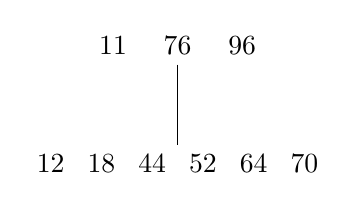
\begin{tikzpicture}[level distance=1.5cm,
  level 1/.style={sibling distance=4cm}]
  
  % Root node
  \node (root) {11 \quad 76 \quad 96}
    child {node[minimum width=3.5cm] (child) {12 \enskip 18 \enskip 44 \enskip 52 \enskip 64 \enskip 70}};
  
\end{tikzpicture}
\end{center}
\end{graybox}

\begin{solution}
\textbf{详细分析:}

\begin{enumerate}
    \item \textbf{分析B树性质:}
    \begin{itemize}
        \item 题目给出的是一个 (3,6)-树,这通常指B树的阶 $m=6$。
        \item 对于一个 $m=6$ 阶的B树,每个节点最多只能包含 $m-1 = 5$ 个关键字。
    \end{itemize}

    \item \textbf{识别上溢:}
    \begin{itemize}
        \item 子节点包含 {12, 18, 44, 52, 64, 70},共6个关键字,这超过了规定的最多5个关键字,因此发生了“上溢”。
    \end{itemize}

    \item \textbf{确定调整策略(分裂):}
    当一个节点发生上溢时,必须进行“分裂”(split)操作。
    \begin{itemize}
        \item \textbf{步骤1:} 从上溢的节点中选取中间的关键字。对于 {12, 18, 44, 52, 64, 70},中间的关键字是 \textbf{44}。
        \item \textbf{步骤2:} 将这个中间关键字 \textbf{44} 提升(promote)到其父节点中,并按序插入。父节点原来的关键字是 {11, 76, 96},插入44后变为 {11, 44, 76, 96}。
        \item \textbf{步骤3:} 将原上溢节点中剩余的关键字分裂成两个新的节点:
            \begin{itemize}
                \item 小于44的关键字形成一个新的左孩子节点:{12, 18}。
                \item 大于44的关键字形成一个新的右孩子节点:{52, 64, 70}。
            \end{itemize}
        \item \textbf{步骤4:} 将这两个新节点链接到父节点,分别位于提升上来的关键字44的两侧。
    \end{itemize}
    经过这个分裂操作,所有节点都重新满足了B树的性质。

\end{enumerate}


\textbf{分裂后的结果为:}
\begin{center}
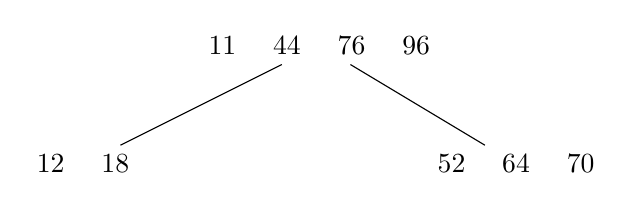
\begin{tikzpicture}[level distance=1.5cm,
  level 1/.style={sibling distance=5cm}]
  
  % Nodes
  \node[minimum width=3cm] (root) {11 \quad 44 \quad 76 \quad 96}
    child[sibling distance=6cm] {node (left) {12 \quad 18}}
    child {node (right) {52 \quad 64 \quad 70}};
    
\end{tikzpicture}
\end{center}
\end{solution}



\section*{140 (版本二)}
\begin{graybox}
下图是(3,6)-树中刚插入节点52后的情形,可以看出发生了上溢,分裂后的结果为(以52为中间关键字):
\begin{center}
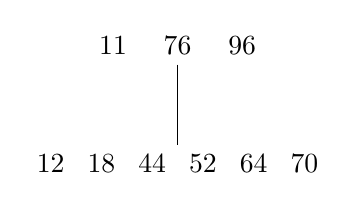
\begin{tikzpicture}[level distance=1.5cm,
  level 1/.style={sibling distance=4cm}]
  
  % Root node
  \node (root) {11 \quad 76 \quad 96}
    child {node[minimum width=3.5cm] (child) {12 \enskip 18 \enskip 44 \enskip 52 \enskip 64 \enskip 70}};
  
\end{tikzpicture}
\end{center}
\end{graybox}

\begin{solution}
\textbf{详细分析:}

\begin{enumerate}
    \item \textbf{分析B树性质:}
    \begin{itemize}
        \item 题目给出的是一个 (3,6)-树,即B树的阶 $m=6$。
        \item 每个节点最多只能包含 $m-1 = 5$ 个关键字。
    \end{itemize}

    \item \textbf{识别上溢:}
    \begin{itemize}
        \item 子节点包含 {12, 18, 44, 52, 64, 70},共6个关键字,超过了最多5个的限制,发生“上溢”。
    \end{itemize}

    \item \textbf{确定调整策略(分裂):}
    当节点上溢时,必须进行“分裂”(split)操作。对于一个有偶数个关键字的节点,中间关键字的选择可以有两种(例如,对于6个关键字,可以选择第3个或第4个)。这里我们按照要求,选择 \textbf{52} 作为提升的中间关键字。
    \begin{itemize}
        \item \textbf{步骤1:} 从上溢的节点中选取中间的关键字 \textbf{52}。
        \item \textbf{步骤2:} 将这个中间关键字 \textbf{52} 提升(promote)到其父节点中,并按序插入。父节点原来的关键字是 {11, 76, 96},插入52后变为 {11, 52, 76, 96}。
        \item \textbf{步骤3:} 将原上溢节点中剩余的关键字分裂成两个新的节点:
            \begin{itemize}
                \item 小于52的关键字形成一个新的左孩子节点:{12, 18, 44}。
                \item 大于52的关键字形成一个新的右孩子节点:{64, 70}。
            \end{itemize}
        \item \textbf{步骤4:} 将这两个新节点链接到父节点,分别位于提升上来的关键字52的两侧。
    \end{itemize}
    经过这个分裂操作,所有节点都重新满足了B树的性质。

\end{enumerate}

\textbf{分裂后的结果为:}
\begin{center}
\begin{tikzpicture}[level distance=1.5cm,
  level 1/.style={sibling distance=6cm}]
  
  % Nodes
  \node[minimum width=3cm] (root) {11 \quad 52 \quad 76 \quad 96}
    child[sibling distance=7cm] {node[minimum width=2.5cm] (left) {12 \quad 18 \quad 44}}
    child {node (right) {64 \quad 70}};
    
\end{tikzpicture}
\end{center}
\end{solution}


\section*{141}
\begin{graybox}
在以下伸展树中插入节点1并经过双层伸展后的结果是:
\begin{center}
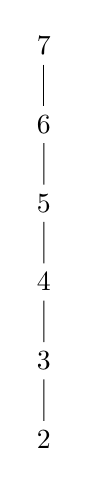
\begin{tikzpicture}[level distance=1cm,
  level 1/.style={sibling distance=1cm},
  level 2/.style={sibling distance=1cm},
  level 3/.style={sibling distance=1cm},
  level 4/.style={sibling distance=1cm},
  level 5/.style={sibling distance=1cm},
  level 6/.style={sibling distance=1cm}]
  
  % Nodes
  \node (7) {7}
    child {node (6) {6}
      child {node (5) {5}
        child {node (4) {4}
          child {node (3) {3}
            child {node (2) {2}}}}}};
\end{tikzpicture}
\end{center}
\end{graybox}

\begin{solution}
\textbf{详细分析:}

\subsection*{第0步:插入节点1}
首先,按照二叉搜索树的规则,将节点1插入为节点2的左孩子。此时,目标节点 \textbf{1} 位于树的最深处。
\begin{center}
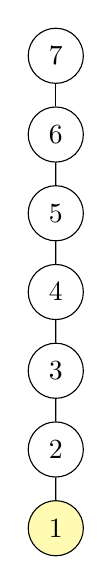
\begin{tikzpicture}[level distance=1cm, level 1/.style={sibling distance=1cm}]
  \node[splaynode] {7}
    child {node[splaynode] {6}
      child {node[splaynode] {5}
        child {node[splaynode] {4}
          child {node[splaynode] {3}
            child {node[splaynode] {2}
              child {node[highlight] {1}}
            }
          }
        }
      }
    };
\end{tikzpicture}
\end{center}

\subsection*{第1轮伸展:Zig-Zig (x=1, p=2, g=3)}
\textbf{1a. 第一次右旋 (围绕 g=3):}
\begin{center}
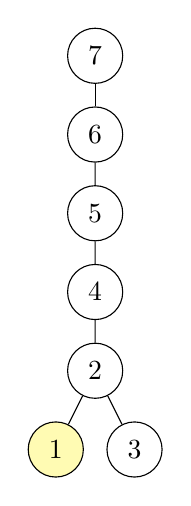
\begin{tikzpicture}[level distance=1cm, level 1/.style={sibling distance=1cm}]
  \node[splaynode] {7}
    child {node[splaynode] {6}
      child {node[splaynode] {5}
        child {node[splaynode] {4}
          child {node[splaynode] {2}
            child {node[highlight] {1}}
            child {node[splaynode] {3}}
          }
        }
      }
    };
\end{tikzpicture}
\end{center}
\textbf{1b. 第二次右旋 (围绕 p=2):}
\begin{center}
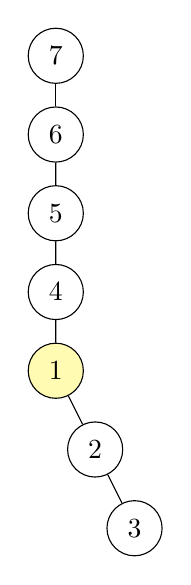
\begin{tikzpicture}[level distance=1cm, level 1/.style={sibling distance=1cm}]
  \node[splaynode] {7}
    child {node[splaynode] {6}
      child {node[splaynode] {5}
        child {node[splaynode] {4}
          child {node[highlight] {1}
            child[missing]
            child {node[splaynode] {2}
              child[missing]
              child {node[splaynode] {3}}
            }
          }
        }
      }
    };
\end{tikzpicture}
\end{center}

\subsection*{第2轮伸展:Zig-Zig (x=1, p=4, g=5)}
\textbf{2a. 第三次右旋 (围绕 g=5):}
\begin{center}
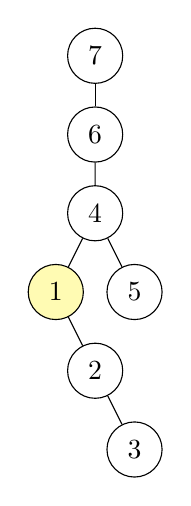
\begin{tikzpicture}[level distance=1cm, level 1/.style={sibling distance=1cm}]
  \node[splaynode] {7}
    child {node[splaynode] {6}
      child {node[splaynode] {4}
        child {node[highlight] {1}
          child[missing]
          child {node[splaynode] {2}
            child[missing]
            child {node[splaynode] {3}}
          }
        }
        child {node[splaynode] {5}}
      }
    };
\end{tikzpicture}
\end{center}

\textbf{2b. 第四次右旋 (围绕 p=4):}
\begin{center}
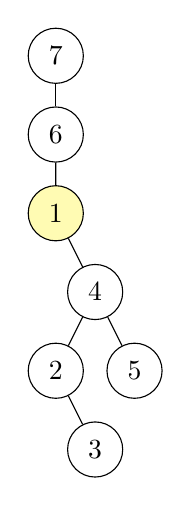
\begin{tikzpicture}[level distance=1cm, level 1/.style={sibling distance=1cm}]
  \node[splaynode] {7}
    child {node[splaynode] {6}
      child {node[highlight] {1}
        child[missing]
        child {node[splaynode] {4}
          child {node[splaynode] {2}
            child[missing]
            child {node[splaynode] {3}}
          }
          child {node[splaynode] {5}}
        }
      }
    };
\end{tikzpicture}
\end{center}

\subsection*{第3轮伸展:Zig-Zig (x=1, p=6, g=7)}
\textbf{3a. 第五次右旋 (围绕 g=7):}
\begin{center}
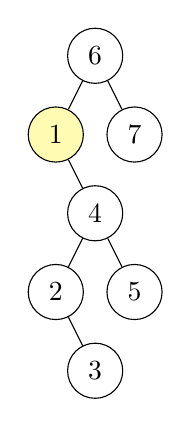
\begin{tikzpicture}[level distance=1cm, level 1/.style={sibling distance=1cm}]
  \node[splaynode] {6}
    child {node[highlight] {1}
      child[missing]
      child {node[splaynode] {4}
        child {node[splaynode] {2}
          child[missing]
          child {node[splaynode] {3}}
        }
        child {node[splaynode] {5}}
      }
    }
    child {node[splaynode] {7}};
\end{tikzpicture}
\end{center}
\textbf{3b. 第六次右旋 (围绕 p=6) - 最终结果:}
\begin{center}
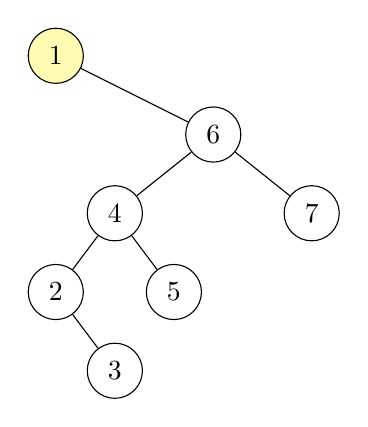
\begin{tikzpicture}[level distance=1cm,
  level 1/.style={sibling distance=4cm},
  level 2/.style={sibling distance=2.5cm},
  level 3/.style={sibling distance=1.5cm}]
  
  \node[highlight] (1) {1}
    child[missing]
    child {node[splaynode] (6) {6}
      child {node[splaynode] (4) {4}
        child {node[splaynode] (2) {2}
          child[missing]
          child {node[splaynode] (3) {3}}
        }
        child {node[splaynode] (5) {5}}
      }
      child {node[splaynode] (7) {7}}
    };
\end{tikzpicture}
\end{center}
\end{solution}

\section*{142(拓展)}
\begin{graybox}
下图是伸展树,其中节点v刚被访问过,双层伸展后的结果是:
\begin{center}
\begin{tikzpicture}[level distance=1.5cm,
  level 1/.style={sibling distance=4cm},
  level 2/.style={sibling distance=2cm}]
  
  % Define rectnode style
  \tikzset{rectnode/.style={draw, rectangle, minimum width=7mm, minimum height=7mm, inner sep=0pt}}

  % Nodes
  \node (p) {p}
    child {node (v) {v}
      child {node[rectnode] (A) {A}}
      child {node[rectnode] (B) {B}}}
    child {node (k) {k}
      child {node[rectnode] (C) {C}}
      child {node[rectnode] (D) {D}}};

\end{tikzpicture}
\end{center}
\end{graybox}

\begin{solution}
\textbf{详细分析:}

\begin{enumerate}
    \item \textbf{分析伸展情况:}
    \begin{itemize}
        \item 被访问的节点是 \textbf{v}。
        \item 节点 \textbf{v} 的父节点是 \textbf{p}。
        \item 父节点 \textbf{p} 是树的根节点,因此节点 \textbf{v} \textbf{没有祖父节点}。
    \end{itemize}

    \item \textbf{确定伸展操作:}
    \begin{itemize}
        \item “双层伸展”(zig-zig 或 zig-zag)只在被访问节点\textbf{存在祖父节点}时执行。
        \item 当被访问节点的父节点就是根节点时,执行的是最简单的“单层伸展”,即 \textbf{zig} 操作。
        \item 在本例中,节点 \textbf{v} 是其父节点 \textbf{p} 的\textbf{左孩子}。因此,需要对父节点 \textbf{p} 执行一次\textbf{右旋转}。
    \end{itemize}

    \item \textbf{执行右旋转(围绕p):}
    \begin{itemize}
        \item 节点 \textbf{v} 上升,成为新的根。
        \item 节点 \textbf{p} 下降,成为 \textbf{v} 的右孩子。
        \item 节点 \textbf{v} 原来的右子树(即子树 \textbf{B})成为 \textbf{p} 的新左孩子。
        \item 节点 \textbf{v} 原来的左子树(即子树 \textbf{A})保持不变,仍是 \textbf{v} 的左孩子。
        \item 节点 \textbf{p} 原来的右子树(即节点 \textbf{k} 和其子树)保持不变,仍是 \textbf{p} 的右孩子。
    \end{itemize}
\end{enumerate}

\textbf{伸展后的结果为:}
\begin{center}
\begin{tikzpicture}[level distance=1.5cm,
  level 1/.style={sibling distance=4cm},
  level 2/.style={sibling distance=3cm},
  level 3/.style={sibling distance=2cm},
  leaf/.style={draw, circle, minimum size=7mm, inner sep=0pt},
  rectnode/.style={draw, rectangle, minimum width=7mm, minimum height=7mm, inner sep=0pt}
  ]
  
  % Nodes
  \node[leaf] (v) {v}
    child {node[rectnode] (A) {A}}
    child {node[leaf] (p) {p}
      child {node[rectnode] (B) {B}}
      child {node[leaf] (k) {k}
        child {node[rectnode] (C) {C}}
        child {node[rectnode] (D) {D}}
      }
    };

\end{tikzpicture}
\end{center}
\end{solution}



\section*{142}
\begin{graybox}
下图是伸展树,其中节点v刚被访问过,双层伸展后的结果是:
\begin{center}
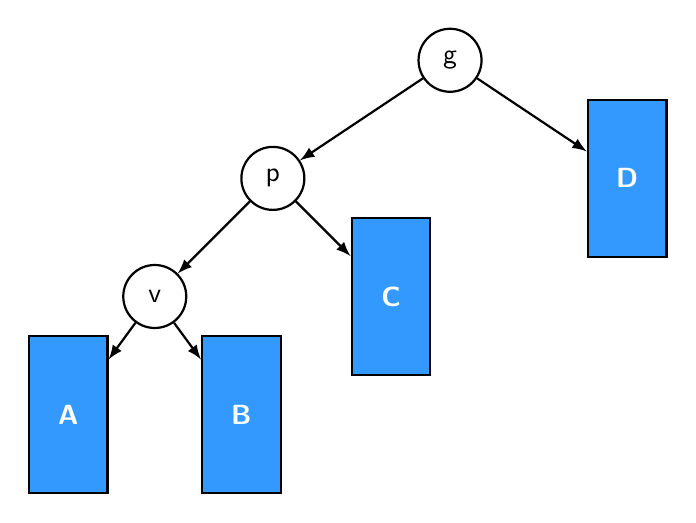
\begin{tikzpicture}[
    % 設定節點間的垂直距離
    level distance=1.5cm,
    % 為不同層級設定節點間的水平距離
    level 1/.style={sibling distance=4.5cm},
    level 2/.style={sibling distance=3cm},
    level 3/.style={sibling distance=2.2cm},
    % 為線條設定樣式
    edge from parent/.style={draw, -latex, thick},
    % --- 定義節點樣式 ---
    % 圓形節點樣式
    circ/.style={
        circle, 
        draw=black, 
        thick, 
        minimum size=8mm, 
        font=\sffamily
    },
    % 長方形節點樣式
    rect/.style={
        rectangle, 
        draw=black, 
        thick, 
        fill=blue!50!cyan!80, % 調整為圖片中的藍色
        text=white, 
        minimum height=2cm, 
        minimum width=1cm, 
        font=\sffamily\bfseries
    }
]

% --- 繪製樹狀結構 ---
% 根節點 g
\node[circ] {g}
    % g 的子節點
    child {
        node[circ] {p}
        % p 的子節點
        child {
            node[circ] {v}
            % v 的子節點
            child { node[rect] {A} }
            child { node[rect] {B} }
        }
        child {
            node[rect] {C}
        }
    }
    child {
        node[rect] {D}
    };

\end{tikzpicture}
\end{center}
\end{graybox}
\begin{solution}
\textbf{详细分析:}

\begin{enumerate}
    \item \textbf{分析伸展情况:}
    \begin{itemize}
        \item 被访问的节点(目标节点)是 \textbf{v}。
        \item \textbf{v} 的父节点是 \textbf{p}。
        \item \textbf{v} 的祖父节点是 \textbf{g}。
    \end{itemize}

    \item \textbf{确定伸展操作:}
    \begin{itemize}
        \item 节点 \textbf{v} 是其父节点 \textbf{p} 的\textbf{左孩子} (zig)。
        \item 节点 \textbf{p} 是其父节点 \textbf{g} 的\textbf{左孩子} (zig)。
        \item 由于两个关系的方向相同(都是左孩子),因此需要执行 \textbf{zig-zig} 操作。
    \end{itemize}

    \item \textbf{执行Zig-Zig操作:}
    Zig-zig操作包含两次同向的旋转。
    \begin{itemize}
        \item \textbf{第一次旋转:} 对祖父节点 \textbf{g} 进行一次右旋转。这会使 \textbf{p} 上升,\textbf{g} 下降成为 \textbf{p} 的右孩子。
        \item \textbf{第二次旋转:} 对(新的)父节点 \textbf{p} 进行一次右旋转。这会使 \textbf{v} 上升,成为新的根。
    \end{itemize}
    
    \item \textbf{重构子树链接:}
    在两次旋转后,为了保持二叉搜索树的性质,四个子树 A, B, C, D 会被重新链接:
    \begin{itemize}
        \item 新的根是 \textbf{v}。
        \item \textbf{v} 的左子树仍然是 \textbf{A}。
        \item \textbf{v} 的右孩子是 \textbf{p}。
        \item \textbf{p} 的左孩子是 \textbf{v} 原来的右子树 \textbf{B}。
        \item \textbf{p} 的右孩子是 \textbf{g}。
        \item \textbf{g} 的左孩子是 \textbf{p} 原来的右子树 \textbf{C}。
        \item \textbf{g} 的右孩子是 \textbf{g} 原来的右子树 \textbf{D}。
    \end{itemize}
\end{enumerate}

\textbf{伸展后的结果为:}
\begin{center}
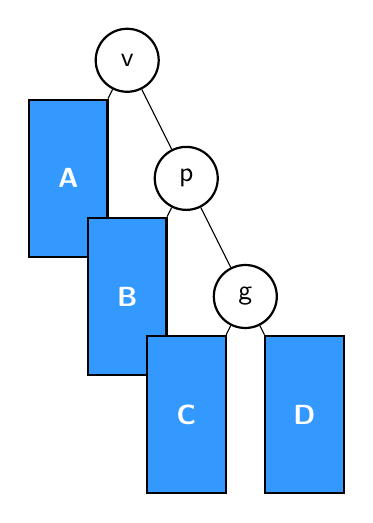
\begin{tikzpicture}[
    circ/.style={
        circle, 
        draw=black, 
        thick, 
        minimum size=8mm, 
        font=\sffamily
    },
    rect/.style={
        rectangle, 
        draw=black, 
        thick, 
        fill=blue!50!cyan!80, 
        text=white, 
        minimum height=2cm, 
        minimum width=1cm, 
        font=\sffamily\bfseries
    }
]
% --- 繪製樹狀結構 ---
% 根節點 v
\node[circ] {v}
    % v 的子節點
    child {
        node[rect] {A}
    }
    child {
        node[circ] {p}
        % p 的子節點
        child {
            node[rect] {B}
        }
        child {
            node[circ] {g}
            % g 的子節點
            child { node[rect] {C} }
            child { node[rect] {D} }
        }
    };
\end{tikzpicture}
\end{center}
\end{solution}
\end{document}

% VScode 常用快捷键:

% Ctrl + R:                 打开最近的文件夹
% F2:                       变量重命名
% Ctrl + Enter:             行中换行
% Alt + up/down:            上下移行
% 鼠标中键 + 移动:           快速多光标
% Shift + Alt + up/down:    上下复制
% Ctrl + left/right:        左右跳单词
% Ctrl + Backspace/Delete:  左右删单词    
% Shift + Delete:           删除此行
% Ctrl + J:                 打开 VScode 下栏(输出栏)
% Ctrl + B:                 打开 VScode 左栏(目录栏)
% Ctrl + `:                 打开 VScode 终端栏
% Ctrl + 0:                 定位文件
% Ctrl + Tab:               切换已打开的文件(切标签)
% Ctrl + Shift + P:         打开全局命令(设置)

% Latex 常用快捷键

% Ctrl + Alt + J:           由代码定位到PDF
% 


% Git提交规范:
% update: Linear Algebra 2 notes
% add: Linear Algebra 2 notes
% import: Linear Algebra 2 notes
% delete: Linear Algebra 2 notes
